\documentclass[../main/main.tex]{subfiles}
\graphicspath{{./figures/}}
\usepackage{pdfpages}

\makeatletter
\renewcommand{\@chapapp}{Travaux pratiques -- TP}
\renewcommand{\chaplett}{TP}
\makeatother

% \toggletrue{student}
% \toggletrue{corrige}
% \renewcommand{\mycol}{black}
% \renewcommand{\mycol}{gray}

\hfuzz=5.002pt

\begin{document}
\setcounter{chapter}{14}

\settype{enon}
\settype{solu_prof}
\settype{solu_stud}

\chapter{\cswitch{Correction du TP}{Analyses spectrales de signaux \'electriques}}

\enonce{%
	\begin{tcn}[sidebyside, sidebyside align=top,
			fontupper=\small, fontlower=\small
		](appl)<ctb>"how"'t'{Capacités exigibles}
		\begin{itemize}[label=\rcheck]
			\item Mettre en œuvre un dispositif expérimental illustrant l'utilité
			      des fonctions de transfert pour un système linéaire à un ou
			      plusieurs étages.
		\end{itemize}
		\tcblower
		\begin{itemize}[label=\rcheck]
			\item Étudier le filtrage linéaire d'un signal non sinusoïdal à partir
			      d'une analyse spectrale.
			\item Détecter le caractère non linéaire d'un système par l'apparition
			      de nouvelles fréquences.
		\end{itemize}
	\end{tcn}
	\vspace{-10pt}
	\section{Objectifs}
	\begin{itemize}
		\item Étudier le filtrage linéaire d'un signal non sinusoïdal à partir
		      d'une analyse spectrale.
		\item Choisir un modèle de filtre en fonction d'un cahier des charges.
	\end{itemize}

	\section{S'approprier~: analyse spectrale}

	\subsection{Décomposition en série de Fourier}

	\begin{tcb}(prop){Décomposition en série de Fourier}
		Toute fonction périodique peut se décomposer en série de Fourier, c'est-à-dire
		en une somme de fonctions sinusoïdales de pulsations différentes. Soit $y$ une
		fonction périodique de période $T$ et de pulsation $\w = 2\pi/T$. La
		décomposition en série de Fourier de $y$ est~:

		\[
			y(t) = y_0 + \sum_{n=1}^{\infty} a_n \cos(n\wt + \f)
		\]

		Avec $a_n$ et $\f_n$ respectivement l'amplitude et la phase de l'harmonique de
		rang $n$.
	\end{tcb}

	% Un logiciel tel que LatisPro (que l'on va utiliser ici) permet de réaliser
	% numériquement la décomposition en série de Fourier (en réalité une transformée
	% de Fourier numérique) d'un signal et de fournir une représentation graphique
	% exploitable.

	\begin{tcb}[sidebyside](exem){}
		\begin{center}
			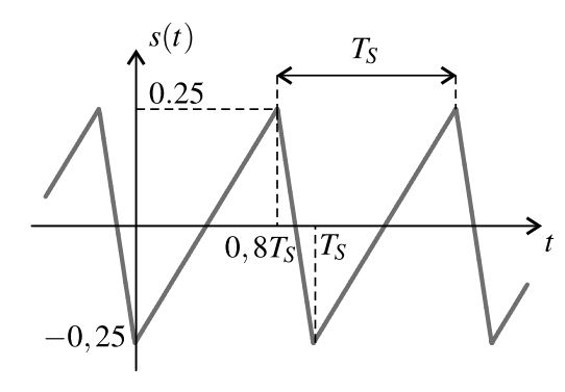
\includegraphics[height=4.5cm]{tp15_spectre-temp}
			\captionof{figure}{Représentation temporelle d'un signal périodique.}
		\end{center}
		\tcblower
		\begin{center}
			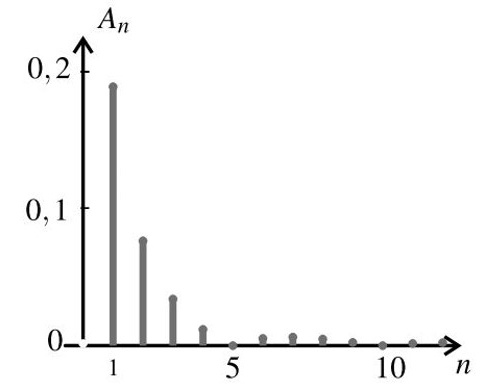
\includegraphics[height=4.5cm]{tp15_spectre-f}
			\captionof{figure}{Spectrogramme du même signal périodique.}
		\end{center}
	\end{tcb}

	\subsection{Vocabulaire}

	\begin{tcb}(nota){Vocabulaire}
		\begin{itemize}
			\item Spectre~: représentation de l'amplitude de chacune des composantes
			      spectrales d'un signal en fonction de leurs pulsations ou de leurs
			      fréquences.
			\item $y_0 = \moy{y(t)}$ est la valeur moyenne du signal $y(t)$,
			      c'est-à-dire sa \textbf{composante continue}~;
			\item $a_1 \cos(\wt + \f_1)$ est appelé
			      \textbf{fondamental}~;
			\item $a_i \cos(n\wt + \f_i)$ est l'\textbf{harmonique} de
			      rang $i$.
		\end{itemize}
	\end{tcb}

	\begin{tcb}(rema)<lftt>'l'{}
		\begin{enumerate}
			\item Le fondamental est aussi l'harmonique de rang $1$.
			\item Le spectre d'un signal temporel pair ne contient que des
			      harmoniques de rang pair ($n=2p, p\in\Nb$)
			\item Le spectre d'un signal temporel impair ne contient que des
			      harmoniques de rang impair ($n=2p+1, p\in\Nb$)
		\end{enumerate}
	\end{tcb}

	\subsection{Durée d'enregistrement et fréquence d'échantillonnage}

	\begin{tcb}(prop){Échantillonnage}
		Le critère de \textsc{Shannon} (vu en seconde année) impose que la
		\textbf{fréquence d'échantillonnage} (fréquence de calcul) soit
		\textbf{supérieure à deux fois la fréquence maximale du signal} étudié.
		\bigbreak
		Par ailleurs, le temps d'acquisition total $T_{\rm acq\, tot}$ doit être égal à
		un multiple entier de fois la période du signal étudié~: $T_{\rm acq\, tot} =
			nT$ avec $n\in \Zb$. Si ce n'est pas possible, il faut que la durée
		d'acquisition soit longue, sachant que le pas fréquentiel du spectre vaudra~:
		\[
			\Delta f = \frac{1}{T_{\rm acq\, tot}}
		\]
	\end{tcb}
}%

\setcounter{section}{2}
\section{Réaliser et valider}
\subsection{Analyses spectrales de signaux périodiques de différentes formes}
\subsubsection{Signal sinusoïdal}

\setlist[blocQR,1]{leftmargin=20pt, label=\clenumi}
\enonce{%
	\begin{tcb}[breakable](expe)<itc>{}
		\underline{Réaliser une acquisition}~:
		\begin{enumerate}
			\item Connecter le générateur basses fréquences (GBF) à l'interface SYSAM
			      entre les voies EA0 et la masse.
			\item Ouvrir le logiciel Latispro en suivant le chemin~: programmes
			      $\rightarrow$ discipline $\rightarrow$ physique-chimie $\rightarrow$
			      latispro.
			\item Allumer le GBF, choisir un signal sinusoïdal de fréquence
			      $\SI{500}{Hz}$ et d'amplitude moyenne ($5-\SI{10}{V}$ par exemple).
			\item Pour faire une acquisition~: cliquer sur le bouton
			      
\includegraphics[height=.5cm]{bouton_acq}
			      \begin{itemize}
				      \item \textit{Pour activer la voie EA0}~: Dans le cadre entrées
				            analogiques, cliquer sur les boutons des entrées à activer (EA0
				            ici~!).
				      \item \textit{Pour paramétrer l'acquisition}~: Dans le cadre
				            acquisition, onglet temporel, mode normal, entrer le nombre de
				            points de mesure et la durée totale de l'acquisition. On
				            choisira~:
				            \begin{itemize}
					            \item Nombre de points~: $\num{10 000}$~;
					            \item Acquisition temporelle~;
				            \end{itemize}
				            \QR{%
					            Durée totale d'acquisition $T_{\rm acq\, tot}$ à
					            choisir. Justifier ce choix succintement.
				            }{%
					            solu
				            }
				            \begin{itemize}
					            \item Fin des réglages, vous êtes prêt-e à faire vos
					                  enregistrements.
				            \end{itemize}
				      \item Lancer l'acquisition en cliquant sur
				            
\includegraphics[height=.5cm]{bouton_lancer}
			      \end{itemize}
		\end{enumerate} \bigbreak

		\underline{Tracer le spectre}~:
		\begin{enumerate}
			\item Aller dans traitements $\rightarrow$ calculs spécifiques $\rightarrow$
			      analyse de Fourier.
			\item Accéder à la liste des courbes gràce à
			      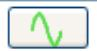
\includegraphics[height=.5cm]{bouton_courbe}
			\item Glisser la courbe et cliquer sur calcul.
		\end{enumerate} \bigbreak
	\end{tcb}
}%

\setlist[blocQR,1]{leftmargin=10pt, label=\sqenumi}
\QR{%
	Quelle est l'allure du spectre~? Observez-vous des harmoniques~?
}{%
	solu
}
\QR{%
	En cliquant droit sur le graphe, prendre la loupe + pour zoomer,
	plusieurs fois si nécessaire ou utiliser le calibrage. Relever la
	fréquence fondamentale grâce à la fonction réticule (toujours en
	cliquant droit sur le graphe) et la comparer à celle indiquée par le
	GBF. Commenter l'éventuelle différence.
}{%
	solu
}

\subsubsection{Signaux triangulaires et carrés}

\enonce{%
	\begin{tcb}(expe)<itc>{}
		Changer la forme du signal délivré par le GBF en gardant la même fréquence
		fondamentale et recommencer le même protocole.
	\end{tcb}
}%

\QR{%
	Quelle est l'allure de chacun des spectres (signal triangulaire et
	carré)~? Observez-vous des harmoniques~?
}{%
	solu
}
\QR{%
	Quelle est la particularité de ces deux spectres~? Quelles sont leurs
	différences~?
}{%
	solu
}

\subsection{Étude du spectre obtenu en sortie du filtre de Rauch}

\enonce{%
	On reprend le filtre de \textsc{Rauch} de la semaine précédente afin de filtrer
	le signal carré~:
	\begin{gather*}
		\boxed{
			\Hu(\jj \w) = \frac{\su}{\eu} = \frac{H_0}{1+\jj Q
				\left(\dfrac{\w}{\w_0}-\dfrac{\w_0}{\w}\right)}
		}
		\\
		\beforetext{Avec}
		Q = \sqrt{\frac{\alpha+1}{2\alpha}},
		\quad
		H_0 = -1
		\qet
		\w_0 = \sqrt{\frac{\alpha+1}{2\alpha}} \, \frac{1}{RC}
	\end{gather*}
	Notre objectif est d'obtenir à partir de ce signal un signal
	sinusoïdal de \textbf{fréquence fondamentale triple}.

	\begin{tcb}(expe)<itc>{Manipulation amplificateur}
		\begin{enumerate}
			\item Connecter la borne \SI{+15}{V} du boitier à la sortie \SI{+15}{V} d'un
			      générateur de tension continue,
			\item Connecter la borne \SI{-15}{V} du boitier à la sortie
			      \SI{-15}{V} du générateur
			\item Connecter le point milieu du boitier à la masse du
			      générateur.
			      \begin{center}
				      \begin{tcb}[cnt,bld,width=.9\linewidth](impo){Attention}
					      À la fin de la séance, on coupe le signal du GBF avant les
					      alimentations de l'amplificateur opérationnel qui doivent être
					      coupées en dernier.
				      \end{tcb}
			      \end{center}
			\item Réalisez ensuite le montage en prenant $C=\SI{1}{nF}$ (cavalier prêt à
			      être connecté sur la boite) et $\alpha R$ avec une boite de résistances
			      variables.
		\end{enumerate}
	\end{tcb}

	On réalise le montage en prenant $C=\SI{1}{nF}$ (cavalier prêt à être connecté
	sur la boite) et $\alpha R$ est une boite de résistances variables. Le filtre a
	été fabriqué avec $R= \SI{100}{k\Omega}$.
	\bigbreak
	On s'intéresse tout d'abord au cas où $\alpha= 1$~: On prend donc $\alpha R =
		\SI{100}{k\Omega}$. On injecte à l'entrée du filtre un signal créneau de
	fréquence fondamentale $f_e$.
}%

\QR{%
	Comment choisir $f_e$ \textit{a priori} afin d'obtenir à partir de ce
	signal un signal sinusoïdal de \textbf{fréquence fondamentale triple}~?
	Choisir cette fréquence sur le GBF.
}{%
	Il faut $f_r = 3f_e$, comme ça seule l'harmonique de rang 3 passe et les
	autres sont atténuées. Or, avec $\alpha = \num{e-2}$, $f_r = f_0 = \SI{11.3}{kHz}$, soit
	\[
		\xul{f_e = \SI{3.8}{kHz}}
	\]
}

\enonce{%
	\begin{tcb}(expe)<itc>{}
		Choisir une durée d'enregistrement telle que $T_{\rm acq\, tot} = 2 T$, ou une
		durée d'enregistrement très grande pour que l'analyse spectrale soit de bonne
		qualité. Faire l'analyse spectrale du signal à l'entrée et à la sortie du
		filtre.
	\end{tcb}
}%

\QR{%
	Qu'observez-vous~? Quelle est l'allure du signal de sortie~?
}{%
	solu
}

\enonce{%
	\begin{tcb}(expe)<itc>{}
		Refaire le même protocole pour $\alpha=\num{e-2}$~: on prend donc $\alpha R =
			\SI{1000}{\Omega}$. On rappelle que la fréquence de résonance trouvée la semaine
		précédente dans ce cas est différente.
	\end{tcb}
}%

\QR{%
	Quelle valeur faut-il alors choisir pour la fréquence fondamentale du
	créneau~? En déduire la valeur à donner à $T_{\rm acq tot}$.
}{%
	De même mais avec $f_0 = \SI{1.5}{kHz}$~:
	\[
		\xul{f_e = \SI{0.5}{kHz}}
		\quad \Lra \quad
		T_e = \frac{1}{f_e} = \SI{2}{ms}
		\quad \Lra \quad
		\xul{T\ind{acq tot} = 2T_e = \SI{4}{ms}}
	\]
}

\section{Conclure}

\QR{%
	Comparez les deux spectres de sortie. Interprétez les différences obtenues.
	Quel filtre permet d'atteindre l'objectif que l'on s'est initialement fixé~?
}{%
	$\alpha = \num{1e-2}$ a une bien plus petite bande passante donc fonctionne
	bien mieux.
}

\end{document}
